\documentclass{article}
\usepackage[UTF8]{ctex}

\usepackage{amsmath}        %数学公式
\usepackage{amssymb}
\usepackage{cases}          %联立编号
\usepackage{cite}           %引用

\usepackage{graphicx}       %插入图片
\usepackage{float}          %设置图片浮动位置
\usepackage{subfigure}      %插入多图时用子图显示

\usepackage{listings}
\usepackage{xcolor}

\usepackage{anyfontsize}    %解决一个奇怪的字体大小报错问题
\usepackage{fancyhdr}       %页眉、页脚、页码
\usepackage[a4paper, margin=1in]{geometry}    %纸张大小
\usepackage{longtable}

\lstset{
    basicstyle          =   \sffamily,          % 基本代码风格
    keywordstyle        =   \bfseries,          % 关键字风格
    commentstyle        =   \rmfamily\itshape,  % 注释的风格,斜体
    stringstyle         =   \ttfamily,  % 字符串风格
    flexiblecolumns,                % 别问为什么,加上这个
    numbers             =   left,   % 行号的位置在左边
    showspaces          =   false,  % 是否显示空格,显示了有点乱,所以不现实了
    numberstyle         =   \zihao{-5}\ttfamily,    % 行号的样式,小五号,tt等宽字体
    showstringspaces    =   false,
    captionpos          =   t,      % 这段代码的名字所呈现的位置,t指的是top上面
    frame               =   lrtb,   % 显示边框
}

\lstdefinestyle{Python}{
    language        =   Python, % 语言选Python
    basicstyle      =   \zihao{-5}\ttfamily,
    numberstyle     =   \zihao{-5}\ttfamily,
    keywordstyle    =   \color{blue},
    keywordstyle    =   [2] \color{teal},
    stringstyle     =   \color{magenta},
    commentstyle    =   \color{red}\ttfamily,
    breaklines      =   true,   % 自动换行,建议不要写太长的行
    columns         =   fixed,  % 如果不加这一句,字间距就不固定,很丑,必须加
    basewidth       =   0.5em,
}

\newcommand\f[2]{\frac{#1}{#2}}
\newcommand\pf[2]{\frac{\partial#1}{\partial#2}}
\newcommand\df[2]{\dfrac{#1}{#2}}
\newcommand\pdf[2]{\dfrac{\partial#1}{\partial#2}}
\newcommand\po[2]{\frac{e^{-#2}#2^#1}{#1!}}

\title{\bf\huge 概率论与数理统计 - 作业 4}
\author{Jerry}
\date{\today}

\begin{document}
\maketitle

\section*{T1. }

恰有两个一点出现的概率$P_1=C_6^2(\f{1}{6})^2(\f{5}{6})^4=\f{3125}{15552}=0.2009$

Possion近似值$P(X=2)=\f{e^{-1}(1)^2}{2!}=\f{1}{2e}\approx0.1839$

\section*{T2. }

$P(X\geq3)=1-(P(X=0)+P(X=1)+P(X=2))$,其中,$P(X=k)=\f{e^{-\lambda}\lambda^k}{k!}$,$\lambda=10^6\cdot p=2$

故$P(X\geq3)=1-(\f{e^{-\lambda}\lambda^0}{0!}+\f{e^{-\lambda}\lambda^1}{1!}+\f{e^{-\lambda}\lambda^2}{2!})=1-e^{-2}(1+2+2)=1-5e^{-2}=0.3233$

\section*{T3. }

由于每次产卵时,它存活与不存活都与其他产卵后是否存活独立,而且产卵事件服从参数为$\lambda$的泊松过程。故只需验证存活的数量$Y$服从均值为$\lambda p$的泊松分布,
即证明:$$P(Y=k)=\f{e^{-\lambda p}(\lambda p)^k}{k!}$$

有$k$个后代的概率
\begin{equation}
    \begin{aligned}
        P(Y=k)
        & =\sum_{0}^{\infty}P(Y=k|X=(k+t))P(X=(k+t))\\
        & =\sum_{0}^{\infty}C_{k+t}^kp^k(1-p)^t\cdot\f{(\lambda t)^{k+t}}{(k+t)^2}e^{-\lambda t}\\
        & =\sum_{0}^{\infty}\f{(\lambda t)^{k+t}}{k!t!}e^{-\lambda t}p^k(1-p)^t\\
        & =\f{e^{-\lambda p}(\lambda p)^k}{k!}\sum_{0}^{\infty}\f{(\lambda p)^t}{t!}e^{-\lambda p}\\
        & =\f{e^{-\lambda p}(\lambda p)^k}{k!}
    \end{aligned}
\end{equation}

得证。

\section*{T4. }

\[
f(x)=
\begin{cases}
    a+bx^2, &\quad 0\leq x \leq1\\
    0, &\quad \text{其他}
\end{cases}
\]

$E(x)=\df{2}{3}$,求$a$,$b$

\begin{equation}
    \begin{aligned}
        \int_{-\infty}^{+\infty}f(x)dx
        & =\int_{0}^{1}(a+bx^2)dx\\
        & =a+\f{b}{3}\\
        & =1
    \end{aligned}
\end{equation}

\begin{equation}
    \begin{aligned}
        E(x)
        & =\int_{-\infty}^{+\infty}xf(x)dx\\
        & =\int_{0}^{1}(a+bx^2)xdx\\
        & =\f{a}{2}+\f{b}{4}\\
        & =\f{2}{3}
    \end{aligned}
\end{equation}

联立(2)(3)式,解得:$a=\f{1}{3}$,$b=2$

\section*{T5. }

\subsubsection*{(1.)}

共计60分钟,其中有20分钟符合不超过10分钟的要求

$P_1=\f{20}{60}=\f{1}{3}$

\subsubsection*{(2.)}

共计60分钟,其中有20分钟符合超过20分钟的要求

$P_2=\f{20}{60}=\f{1}{3}$

\section*{T6. }

正态分布的$\sigma$区间内概率是0.6826,故$P(|X-\mu|\leq\sigma)=0.6826$

正态分布的$2\sigma$区间内概率是0.9544,故$P(|X-\mu|\leq2\sigma)=0.9544$

正态分布的$3\sigma$区间内概率是0.9974,故$P(|X-\mu|\leq3\sigma)=0.9974$

出生前290天位于$\mu+2\sigma$,出生前240天位于$\mu-3\sigma$

故有过长或过短的怀孕期的概率为$1-(\f{0.9544}{2}+\f{0.9974}{2})=0.0238$

\section*{T7. }

\subsubsection*{(1.)}

电池的损耗为指数分布且期望为$30000$,则

$P(15000\leq X\leq25000)=\int_{15000}^{25000}\f{1}{30000}e^{-\f{x}{30000}}dx=0.3297$

\subsubsection*{(2.)}

当知道分布函数$F$时,我们可以求出概率密度函数$f$,即$f(x)=F'(x)$

$P(15000\leq X\leq25000)=\int_{15000}^{25000}f(x)dx=\int_{15000}^{25000}F'(x)dx=F(25000)-F(15000)$

\section*{T8. }

对无罪的人,概率累计分布函数$P_1(x)=1-e^{-x}$

对有罪的人,概率累计分布函数$P_2(x)=1-e^{-\f{1}{2}x}$

\subsubsection*{(1.)}

95\%的概率不冤枉无罪的人,即$P_1(x)\geq0.95$,解得$x\geq2.9957$

\subsubsection*{(2.)}

计算将一个确实有罪的被告判为有罪的概率$P_2(x)=1-(1-e^{-\f{1}{2}x})=e^{-\f{1}{2}\cdot 2.9957}=0.0500$

\section*{T9. }

$Y>0$,$\ln Y$\~{}$N(\mu, \sigma^2)$

则$p(\ln Y)=\f{1}{\sigma\sqrt{2\pi}}e^{-\f{(\ln Y-\mu)^2}{2\sigma^2}}$

$P(\ln Y<X)=\int_{-\infty}^{X}\f{1}{\sigma\sqrt{2\pi}}e^{-\f{(\ln Y-\mu)^2}{2\sigma^2}}d(\ln Y)=\int_{-\infty}^{X}\f{1}{\sigma\sqrt{2\pi}}e^{-\f{(\ln Y-\mu)^2}{2\sigma^2}}\f{1}{Y}dY$

$p(Y)=\f{1}{\sigma\sqrt{2\pi}}e^{-\f{(\ln Y-\mu)^2}{2\sigma^2}}\f{1}{Y}$

\section*{T10 .}

随机变量$X$的累积分布函数为$F(x)$,$F(x)$连续且严格单调

\subsubsection*{(1.)}

% $p(y)=f(g^{-1}(y))|[g^{-1}(y)]'|$

$P(Y\leq y)=P(g(X)\leq y)=P(X\leq g^{-1}(y))=F(g^{-1}(y))$

$F(g^{-1}(y))=y$,即$g^{-1}(y)=F^{-1}(y)$

$p(y)=f(F^{-1}(y))|[F^{-1}(y)]'|=\f{f(F^{-1}(y))}{F'(F^{-1}(y))}$

\subsubsection*{(2.)}

$P(Y\leq y)=P(F(X)\leq y)=P(X\leq F^{-1}(y))=F(F^{-1}(y))=y$

\subsubsection*{(3.)}

% $Y$\~{}$U(0,1)$,则$F(x)=P(Y\leq F(X))=P(F^{-1}(Y)\leq X)=P(Y\leq y)=F(y)$

$F^{-1}(Y)$的累积分布函数为$F(x)$,即$P(F^{-1}(Y)\leq x)=F(x)$,其中$F^{-1}$为$F$的反函数,$F$为指数分布的累积分布函数,
$F(x)=1-e^{-\lambda x}$,$F^{-1}(x)=-\f{\ln(1-x)}{\lambda}$,$F^{-1}(Y)=-\f{\ln(1-Y)}{\lambda}$,$P(F^{-1}(Y)\leq x)=
P(-\f{\ln(1-Y)}{\lambda}\leq x)=P(Y\leq 1-e^{-\lambda x})=F(x)$,得证。

\subsubsection*{(4.)}

用于生成指定概率密度的随机变量

\subsubsection*{(5.)}

不正确,因为此时$F^{-1}(y)$不一定存在

\section*{T11. }

\subsubsection*{(1.)}

\[
Y=
\begin{cases}
    1, &\quad p_1\\
    2, &\quad p_2\\
    \dots\\
    i, &\quad p_i\\
    \dots\\
    n, &\quad p_n
\end{cases}
\]

\subsubsection*{(2.)}

将一个连续的均匀分布的随机变量均匀的映射到一个单位长度的线段上,再将这个线段按照概率分段,即可将一个连续的均匀分布的随机变量转换成一般的离散性随机变量

\section*{T12. }

我们认为随机断开为在线段上取一个点$t$,将线段分为$[0,t]$与$(t,1]$两个部分

当$t\geq p$时,$[0,t]$部分包含$p$,当$t<p$时,$(t,1]$部分包含$p$

计算包含$p$线段长度的期望:

$E(X)=\int_{0}^{p}tdt+\int_{p}^{1}(1-t)dt=\f{p^2}{2}+\f{1}{2}-p$

\section*{T13. }

硬币的正反面是等概率的,都是$\f{1}{2}$。我们考虑所有事件,当正面时服从(0,1)上的均匀分布,当反面时服从(3,4)上的均匀分布。

期望$E(X)=\f{1}{2}\int_{0}^{1}xdx+\f{1}{2}\int_{3}^{4}xdx=\f{7}{2}$

方差$Var(X)=E(X^2)-(E(X))^2=\f{1}{2}\int_{0}^{1}x^2dx+\f{1}{2}\int_{3}^{4}x^2dx-(\f{7}{2})^2=\f{1}{3}$

\section*{T14. }

$\beta$分布的概率密度函数是:

\begin{equation}
    \begin{aligned}
        f(x;\alpha,\beta)
        & = \f{x^{\alpha-1}(1-x)^{\beta-1}}{\int_{0}^{1}u^{\alpha-1}(1-u)^{\beta-1}du}\\
        & = \f{\Gamma(\alpha+\beta)}{\Gamma(\alpha)+\Gamma(\beta)}x^{\alpha-1}(1-x)^{\beta-1}\\
        & = \f{1}{B(\alpha,\beta)}x^{\alpha-1}(1-x)^{\beta-1}
    \end{aligned}
\end{equation}

其中,$B(\alpha,\beta)=\f{\Gamma(\alpha)\Gamma(\beta)}{\Gamma(\alpha+\beta)}$,$\Gamma(x)=\int_{0}^{+\infty}u^{x-1}e^{-u}du$

$x$的数学期望为

\begin{equation}
    \begin{aligned}
        E(X)
        & = \int_{0}^{1}xf(x;\alpha,\beta)dx\\
        & = \int_{0}^{1}x \f{1}{B(\alpha,\beta)}x^{\alpha-1}(1-x)^{\beta-1}dx\\
        & = \f{1}{B(\alpha,\beta)}\int_{0}^{1}x^{\alpha}(1-x)^{\beta-1}dx\\
        & = \f{B(\alpha+1,\beta)}{B(\alpha,\beta)}\\
        & = \f{\Gamma(\alpha+1)\Gamma(\beta)}{\Gamma(\alpha+\beta+1)}\f{\Gamma(\alpha+\beta)}{\Gamma(\alpha)\Gamma(\beta)}\\
        & = \f{\alpha}{\alpha+\beta}
    \end{aligned}
\end{equation}

$x^2$的数学期望为

\begin{equation}
    \begin{aligned}
        E(X^2)
        & = \int_{0}^{1}x^2f(x;\alpha,\beta)dx\\
        & = \int_{0}^{1}x^2 \f{1}{B(\alpha,\beta)}x^{\alpha-1}(1-x)^{\beta-1}dx\\
        & = \f{1}{B(\alpha,\beta)}\int_{0}^{1}x^{\alpha+1}(1-x)^{\beta+1}dx\\
        & = \f{B(\alpha+2,\beta)}{B(\alpha,\beta)}\\
        & = \f{\Gamma(\alpha+2)\Gamma(\beta)}{\Gamma(\alpha+\beta+2)}\f{\Gamma(\alpha+\beta)}{\Gamma(\alpha)\Gamma(\beta)}\\
        & = \f{(\Gamma(\alpha)(\alpha+1)\alpha)\Gamma(\beta)}{\Gamma(\alpha+\beta)(\alpha+\beta+1)(\alpha+\beta)}\f{\Gamma(\alpha+\beta)}{\Gamma(\alpha)\Gamma(\beta)}\\
        & = \f{\alpha(\alpha+1)}{(\alpha+\beta)(\alpha+\beta+1)}
    \end{aligned}
\end{equation}

方差为

\begin{equation}
    \begin{aligned}
        Var(X)
        & = E(X^2)-E(X)^2\\
        & = \f{\alpha(\alpha+1)}{(\alpha+\beta)(\alpha+\beta+1)}-\f{\alpha^2}{(\alpha+\beta)^2}\\
        & = \f{\alpha\beta}{(\alpha+\beta)^2(\alpha+\beta+1)}
    \end{aligned}
\end{equation}

\section*{T15. }

\subsubsection*{(1.)}

\begin{center}
    \begin{figure}[H] %H为当前位置,!htb为忽略美学标准,htbp为浮动图形
        \centering %图片居中
        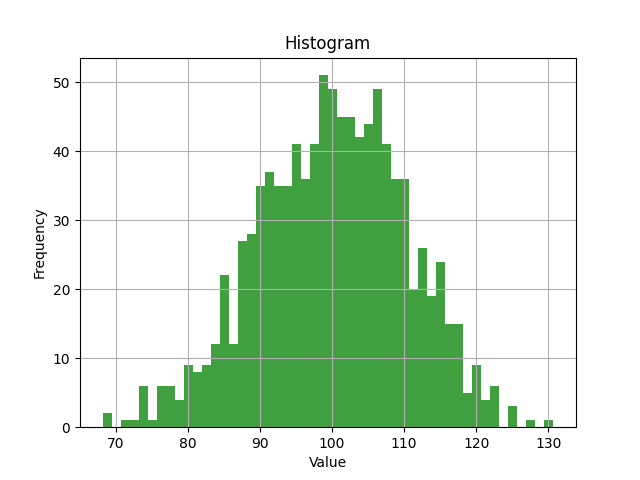
\includegraphics[width=0.45\textwidth]{img/Figure_1.png} %插入图片,[]中设置图片大小,{}中是图片文件名
        \caption{正态分布} %最终文档中希望显示的图片标题
        \label{fig1} %用于文内引用的标签
    \end{figure}
\end{center}

\subsubsection*{(2.)}

\begin{center}
    \begin{figure}[H] %H为当前位置,!htb为忽略美学标准,htbp为浮动图形
        \centering %图片居中
        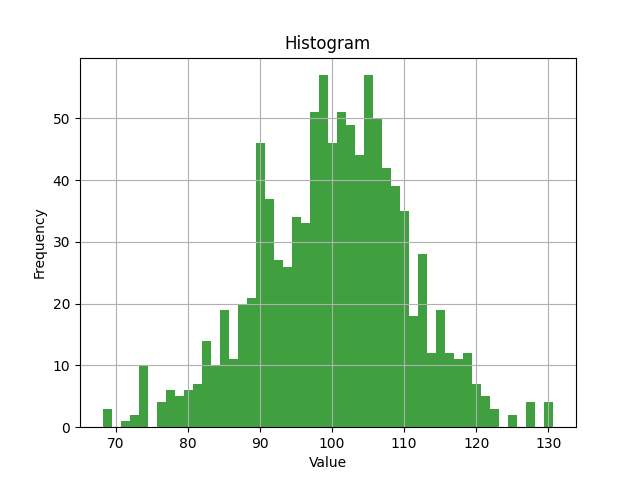
\includegraphics[width=0.45\textwidth]{img/Figure_2.png} %插入图片,[]中设置图片大小,{}中是图片文件名
        \caption{随机抽取} %最终文档中希望显示的图片标题
        \label{fig2} %用于文内引用的标签
    \end{figure}
\end{center}

\subsubsection*{(3.)}

正态分布的均值: 100.04370007177603

随机抽取的均值:100.23370675880342

正态分布的方差: 105.50725243237409

随机抽取的方差: 106.9221614415005

\subsubsection*{Code}

源代码如下:

\lstinputlisting[
    style       =   Python,
    caption     =   {\bf simulation1.py},
    label       =   {1}
]{code/simulation1.py}

除图像外运行结果如下:

E(X) of data: 100.04370007177603

Var(X) of data: 105.50725243237409

E(X) of new\_data: 100.23370675880342

Var(X) of new\_data: 106.9221614415005

\end{document}
